\documentclass[english,russian,a4paper,12pt]{article}
\usepackage[utf8x]{inputenc}
\usepackage[T2A]{fontenc}
\usepackage{babel}
\usepackage{csquotes}

\usepackage{fullpage}
\usepackage{indentfirst}
\usepackage[font=small,labelfont=bf,labelsep=period]{caption}

\usepackage{amssymb, amsmath}
\usepackage{wrapfig}
\usepackage{graphicx}
\usepackage{movie15}

\newcommand{\dd}{\:\mathrm{d}}
\newcommand{\Kn}{\mathrm{Kn}}
\newcommand{\D}{\mathrm{d}}

\usepackage[
	pdfauthor={Oleg Rogozin},
	pdftitle={Couette Flow and Heat Transfer between Two Parallel Plates},
	colorlinks,pdftex,unicode]{hyperref}
\hypersetup{linkcolor=blue}
\newcommand{\HRule}{\rule{\linewidth}{0.5mm}}

\begin{document}
\noindent\HRule\\
 УДК 533.72
\begin{center}
	\large\textbf{Рогозин О.А.}\textsuperscript{1}\\
	\bf\huge Течение Куэтта и перенос тепла между двумя параллельными пластинами
\end{center}
\HRule\\
\textsuperscript{1} Московский физико"=технический институт


\section*{\centeringВведение}

Одномерные задачи течения Ку\'{э}тта и переноса тепла между двумя параллельными пластинами являются наиболее простыми,
но основополагающими в динамике разреженного газа. В работе изучаются линейные приближения задач,
которые соответствуют малым градиентам макропараметров. В такой постановке они хорошо изучены
для всего диапазона чисел Кнудсена и при этом подробно табулированы с высокой точностью~[\ref{bib:dXXX-1},~\ref{bib:dXXX-2}].
Целью работы является верификация проекционного метода решения кинетического уравнения Больцмана~[\ref{bib:dXXX-3}]
на основе точного решения линеаризованного приближения.

\section*{\centeringПостановка задачи}

Рассмотрим одноатомный идеальный газ между двумя бесконечными параллельными пластинами с полным диффузным отражением.
Ось абсцисс направлена перпендикулярно пластинам, расстояние между которыми равно \(L\).
В качестве молекулярного потенциала взаимодействия выберем модель твердых сфер.

Течение Куэтта образуется при  относительном движении пластин друг относительно друга с продольной скоростью \(U\)
вдоль оси ординат, при этом плотность газа \(\rho\) и температура стенок и газа \(T\) остаются постоянными.
В стационарном состоянии уставливается константный профиль сдвигового напряжения \(p_{xy}\).

Задача переноса тепла ставится для фиксированного отношения температур покоящихся стенок \(T_1>T_2\),
при котором уставливается константный профиль теплового потока \(q_x\).

\section*{\centeringБезразмерные переменные}

В работе будем придерживаться современных обозначений, принятых 
в классической монографии Соуна <<Молекулярная динамика>>~[\ref{bib:dXXX-2}].
Безразмерные величины будем отмечать символом <<шляпки>>.

Микроскопические величины в уравнении Больцмана
\[
	\frac{\partial{f}}{\partial{t}} + \xi_i\frac{\partial{f}}{\partial X_i} = 
	\int (f'f'_1-ff_1)|\boldsymbol{\xi}-\boldsymbol{\xi}'|b\dd b \dd \varepsilon \boldsymbol{\dd\xi},
\]
такие как координата \(X_i\), скорость \(\xi_i\), время \(t\), прицельное расстояние \(b\)
и функция распределения \(f\) принимают безразмерный вид согласно формулам:
\[ f = \hat{f}f_0,\; \xi_i = \zeta_i\nu_0,\; X_i = x_i\ell_0,\;
	t = \hat{t}\frac{\ell_0}{\nu_0},\; b = \hat{b}d_m \]
Для макроскопических параметров, таких как плотность \( \rho = \hat{\rho}\rho_0\), макроскопическая скорость \(v_i = \hat{v}_iv_0\),
температура \(T = \hat{T}T_0\), тензор напряжений \(p_{ij} = \hat{p}_{ij}p_0\) и тепловой поток \(q_i = \hat{q}_iq_0\), 
безразмерные соотношения определим естественным образом:
\[ \rho_0 = f_0 \nu_0^3, \; v_0 = \nu_0, \; p_0 = \rho_0RT_0, \; q_0 = p_0\nu_0, \]
где \(R = k_B/m\) "--- удельная газовая постоянная, равная отношению постоянной Больцмана \(k_B\) к молекулярной массе \(m\).
Значения \(\rho_0\) и \(T_0\) выбирались как средние плотность и температура соответственно,
в частности для задачи переноса тепла \(T_0 = (T_1+T_2)/2\).

Наконец, свяжем две единицы измерения длины \(x\), \(b\) и единицы температуры \(T_0\), скорости \(\nu_0\):
\[ \ell_0 = \frac{m}{\pi\sqrt2 \rho_0 d_m^2}, \; \nu_0 = 2RT_0, \]
так что \(\ell_0\) окажется длиной свободного пробега, \(d_m\) "--- эффективным диаметром молекул газа,
а \(\nu_0\) "--- средней тепловой скоростью газа.

Итак, в безразмерных переменных кинетическое уравнение Больцмана примет вид
\[ \frac{\partial\hat{f}}{\partial\hat{t}} + \zeta_i\frac{\partial\hat{f}}{\partial x_i} = \hat{J}(\hat{f},\hat{f}), \]
\[ 
	\hat{J}(\hat{f},\hat{f}) = \frac1{\pi\sqrt2}\int (\hat{f'}\hat{f'_1}-\hat{f}\hat{f_1})
	|\boldsymbol{\zeta}-\boldsymbol{\zeta}'| \hat{b}\dd \hat{b} \dd \varepsilon \boldsymbol{\dd\zeta},
\]
а макропараметры будут вычиляться по формулам:
\begin{alignat*}{2}
	\hat{\rho} &= \int \hat{f}\boldsymbol{\dd\zeta}, \\
	\hat{\rho}\hat{v}_i &= \int \zeta_i \hat{f}\boldsymbol{\dd\zeta}, \\
	\frac3{2}\hat{\rho}\hat{T} &= \int(\zeta_i-\hat{v}_i)^2\hat{f}\boldsymbol{\dd\zeta}, \\
	\frac1{2}\hat{p}_{ij} &= \int(\zeta_i-\hat{v}_i)(\zeta_j-\hat{v}_j)\hat{f}\boldsymbol{\dd\zeta}, \\
	\hat{q}_i &= \int(\zeta_i-\hat{v}_i)(\zeta_j-\hat{v}_j)^2\hat{f}\boldsymbol{\dd\zeta}.
\end{alignat*}

Давление вычисляется как \(\hat{p} \equiv \hat{p}_{ii}/3 = \hat{\rho}\hat{T}\), а число Кнудсена будем определять как \(\Kn=\ell_0/L\).
Аналогично можно записать безразмерные коэффициенты вязкости \(\mu\) и теплопроводности \(\lambda\):
\[ \mu = \hat{\mu}\rho\nu\ell = \hat{\mu}\sqrt{\hat{T}}\mu_0, \; \mu_0 = \rho_0\nu_0\ell_0, \]
\[ \lambda = \hat{\lambda}R\rho\nu\ell = \hat{\lambda}\sqrt{\hat{T}}\lambda_0, \; \lambda_0 = R\rho_0\nu_0\ell_0. \]
 
\section*{\centeringМетодика численного решения уравнения Больцмана}

Кинетическое уравнение Больцмана решалось симметричным методом расщепления на уравнение переноса
\[ \frac{\partial\hat{f}}{\partial\hat{t}} + \zeta_i\frac{\partial\hat{f}}{\partial x_i} = 0, \]
для которого использовалась консервативная TVD схема с ограничителем третьего порядка аппроксимации~[\ref{bib:dXXX-4}],
и уравнение релаксации
\[ \frac{\partial\hat{f}}{\partial\hat{t}} = \hat{J}(\hat{f},\hat{f}), \]
которое в свою очередь решалось проекционным методом~[\ref{bib:dXXX-3}].

В качестве дискретного пространства скоростей использовался шар радиусом \footnote
{
	4.3 тепловых скорости достаточно, чтобы обеспечить точность 0.01\% совпадения
	первых тринадцати моментов функции распределения (малой величины) с соответствующими разностными аналогами.
}\(4.3\nu_0\),
равномерно заполненный узлами так, что на радиусе помещалось 16 точек.
Одномерное координатное пространство состояло как минимум из 30 одинаковых кубических ячеек,
при условии что их размер не превышал единицы.

Для взятия интеграла столкновений применялись сетки Коробова размером от 0.1 до 1 млн. точек.
Стационарные значения макропараметров усредненялись на последних 500 временных итераций,
что обеспечивало точность не ниже 0.1\%.

Для ускорения расчётов в качестве начальной функции распределения выбиралось тринадцатимоментное приближение Грэда
\[ 
	\hat{f}_{G13} = \frac{\hat\rho}{(\pi\hat T)^{3/2}}\exp\left(-\frac{c_i^2}{\hat T}\right)
	\left( 1+\frac{\hat p_{ij}c_ic_j}{\hat p\hat T} + \frac4{5}\frac{\hat q_ic_i}{\hat p\hat T}\left(\frac{c_i^2}{\hat T}-\frac5{2}\right) \right),
	\quad c_i = \zeta_i - \hat v_i
\]
с соответствующими точному решению профилями макропараметров.

В задаче Куэтта относительная скорость пластин равнялась \(\hat{U}=0.01\),
и такое же значение отношения температур \(\hat{T}_1/\hat{T}_2\) использовалось в задаче теплопереноса.
Этого достаточно, чтобы обеспечить линейность задачи с точностью порядка 0.01\%.

\section*{\centeringРезультаты}

\subsection*{\centeringТечение Куэтта}

Для задачи Куэтта сравнивались зависимости сдвигового напряжения (рис.~\ref{fig:couette:shear}),
потоков массы (рис.~\ref{fig:couette:flow}) и тепла (рис.~\ref{fig:couette:qflow})
через половину сечения от числа Кнудсена.

В рамках линейной теории для бесстолкновительного газа
\[ \frac{\hat{p}_{xy}}{\hat{U}} = -\frac1{\sqrt{\pi}}, \]
а при небольших \(\Kn\) справедливо асимптотическое решение\footnote
{ Получается при решении уравнения Больцмана методом Грэда"--~Гильберта~[\ref{bib:dXXX-2}]: разложение по малому параметру \(\Kn\). }
\[ \frac{\hat{p}_{xy}}{\hat{U}} = \frac{2\hat{\mu}\Kn}{1-\sqrt{\pi}k_0\Kn}. \]
Коэффициенты вязкости \(\hat{\mu}\) и скольжения \(k_0\) для модели твёрдых сфер равны~[\ref{bib:dXXX-2}]
\[ \hat{\mu} = 0.562773, \; k_0 = -1.2540. \]
Отбросив знаменатель, получим гидродинамическое решение \(\hat{p}_{xy} = 2\hat{\mu}\Kn\hat{U}\).
Численные значения точного решения табулированы в~[\ref{bib:dXXX-1}].

Кроме того, для сравнения представлены некоторые результаты 
решения модельного кинетического уравнения БКВ (Больцмана"--~Крука"--~Веландера).
Несмотря на хорошое совпадение модельного решения с точным для значения сдвигового напряжения,
метод БКВ даёт значительную погрешность для потоков массы и тепла~[\ref{bib:dXXX-2}],
поэтому они даже не приводятся на соответствующих графиках.

\begin{figure}
	\centering
	\includegraphics{couette/graph.pdf}
	\caption{Зависимость сдвигового напряжения от числа Кнудсена}\label{fig:couette:shear}
\end{figure}

\begin{figure}
	\centering
	\includegraphics{couette/flow.pdf}
	\caption{Зависимость потока массы через половину сечения от числа Кнудсена}\label{fig:couette:flow}
\end{figure}

\begin{figure}
	\centering
	\includegraphics{couette/qflow.pdf}
	\caption{Зависимость потока тепла через половину сечения от числа Кнудсена}\label{fig:couette:qflow}
\end{figure}

На рис.~\ref{fig:couette:shear} наблюдается хорошое совпадение результатов.
Однако для бесстолкновительного газа заметно превышение \(\hat{p}_{xy}\) на 0.61\%,
что может быть обусловлено только ошибкой дискретной аппроксимации разрывной функции распределения по скоростному пространству.
При интерполяции полученной кривой на интервале \(\Kn\in[0,0.2]\) асимптотическим решением 
можно произвести подбор параметров нелинейным методом наименьших квадратов.
С его помощью в области континуального описания газа определяется оклонение 
от коэффициентов вязкости (\(+0.83\%\)) и скольжения (\(-1.2\%\)).

На рис.~\ref{fig:couette:flow},~\ref{fig:couette:qflow} для сильно разреженного газа наблюдаются значительные отклонения,
которые объясняются плохой работоспособностью метода дискретных ординат в соответствующей области чисел Кнудсена.

\subsection*{\centeringПеренос тепла}

Для задачи переноса тепла проанализируем зависимость теплового потока \(q\) от числа Кнудсена (рис.~\ref{fig:heat}).

В рамках линейной теории для бесстолкновительного газа
\[ \frac{\hat{q}_x}{\hat{T}_1-\hat{T}_2} = -\frac1{\sqrt{\pi}}, \]
а при небольших \(\Kn\) справедливо асимптотическое решение
\[ \frac{\hat{q}_x}{\hat{T}_1-\hat{T}_2} = -\frac{\hat{\lambda}\Kn}{1+\sqrt{\pi}d_1\Kn}. \]
Коэффициенты теплопроводности \(\hat{\lambda}\) и скачка температуры на стенке \(d_1\) для модели твёрдых сфер равны~[\ref{bib:dXXX-2}]
\[ \hat{\lambda} = 2.129475, \; d_1 = 2.4001. \]
Отбросив знаменатель, получим гидродинамическое решение \(\hat{q}_x = -\hat{\lambda}\Kn(\hat{T}_1-\hat{T}_2)\).
Численные значения точного решения табулированы в~[\ref{bib:dXXX-2}].

\begin{figure}
	\centering
	\includegraphics{heat/graph.pdf}
	\caption{Зависимость теплового потока от числа Кнудсена}\label{fig:heat}
\end{figure}

Как и в задаче о течении Куэтта, на рис.~\ref{fig:heat} видна хорошая сходимость к точному решению,
однако одновременно наблюдаются те же проблемы: завышение значений теплопотока на \(0.63\)\%
для бесстолкновительного газа и значительная ошибка в коэффициенте теплопроводности (\(+2.2\%\)).
По всей видимости, последняя объясняется неточной аппроксимацией угла разлёта сталкивающихся молекул,
в частности, существованием минимально разрешимого угла разлёта.

\subsection*{\centeringИсследование погрешности}

Логичным представляется исследование зависимости указанных погрешностей от числа интерполирующих узлов
скоростного пространства. Будем анализировать ошибки аппроксимации задачи переноса тепла.
Для этого коэффициент теплопроводности вычислялся локально в точке \(x_0=\hat L/2\) по формуле
\[ \hat{q_x}(x_0) = -\hat{\lambda}\frac{\D\hat T}{\D x}\bigg|_{x=x_0}. \]

Соответствующие графики в логарифмическом масштабе представлены на рис.~\ref{fig:error}.
Наклон прямых говорит примерно о квадратичной зависимости:
\[ \varepsilon \propto R_\Omega^{-2} \propto V_\Omega^{-2/3}, \]
где \(R_\Omega\) "--- число узлов на радиусе скоростной сетки, \(V_\Omega\) "--- её объём.

При \(R_\Omega = 40\) точность вычисления теплового потока повышается до \(0.1\%\),
а коэффициента теплопроводности только до \(0.5\%\).

\begin{figure}
	\centering
	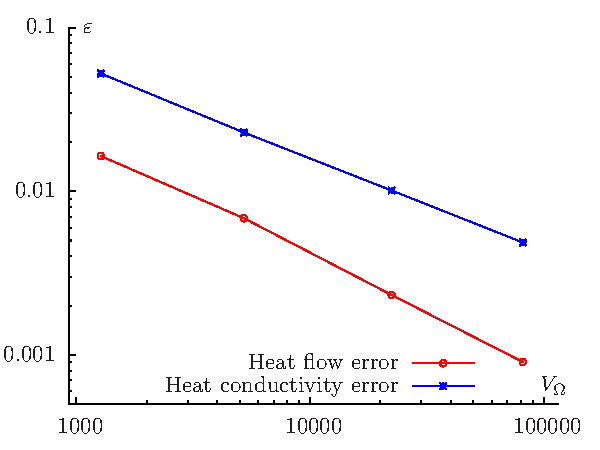
\includegraphics{error/error.pdf}
	\caption{
		Зависимость от числа узлов на радиусе скоростной сетки погрешностей вычисления 
		теплопотока для бесстолкновительного газа и коэффициента теплопроводности для слаборазреженного газа
	}\label{fig:error}
\end{figure}

\section*{\centeringЗаключение}

Показана удовлетворительная сходимость численного решения уравнения Больцмана проекционным методом
простейших одномерных линейных задач: течения Куэтта и переноса тепла --- к эталонным на основе
линеаризованного уравнения.

Выявлены две проблемы. Во-первых, медленная сходимость погрешности аппроксимации макропараметров по отношению к
объёму используемой оперативной памяти вычислительной системы. Возможным решением является корректировка всех значений макропараметров
по их отклонению в бесстолкновительном режиме при используемом \(R_\Omega\) от некоторого большего \(R_\Omega\),
при котором результаты можно считать достоверными.

Во-вторых, существенна погрешность в определении коэффициентов вязкости и особенно теплопроводности.
По всей видимости, качественно улучшить аппроксимацию межмолекулярного потенциала позволит лишь использование
более чем двухточечного проекционного метода, который обеспечит точное значение угла разлёта.
Эта идея впервые выдвинута \fbox{Бейлихом}~[\ref{bib:dXXX-5}].

\section*{\centeringЛитература}

\begin{enumerate}
	\item \textit{Y. Sone, S. Takata and T. Ohwada.}
	Numerical analysis of the plane Couette flow of a rarefied gas on the basis of the linearized Boltzmann equation
	for hard"=sphere molecules. -- European Journal of Mechanics B Fluids. -- 1990. -- N.~8. -- P.~273--288.\label{bib:dXXX-1}
	\item \textit{Y. Sone.}
	Molecular gas dynamics: theory, techniques, and applications. -- Birkhauser, 2007. -- P.~658. \label{bib:dXXX-2}
	\item \textit{F. Tcheremissine.}
	Conservative evaluation of Boltzmann collision integral in discrete ordinates approximation. --
	Computers \& Mathematics with Applications. -- 1998. -- V.~38, N.~1-2. -- P.~215--221. \label{bib:dXXX-3}
	\item \textit{Рогозин О.А.} Сравнение TVD"=ограничителей.
	// Труды 50-й научной конференции МФТИ <<Современные проблемы фундаментальных и прикладных наук>>.
	2010. Т.~2. -- С. 97--98. \label{bib:dXXX-4}
	\item \textit{A.E. Beylich.}
	Solving the kinetic equation for all Knudsen numbers. --
	Physics of Fluids. -- 2000. -- V.~12, N.~2. -- P.~444--465. \label{bib:dXXX-5}
	
\end{enumerate}

\end{document}
